\chapter{Introduction} \label{chp:intro}
    
    \section{Motivation}

        In 2016, \textcite{lubinRoadmapInterstellarFlight2016} proposed sending \qty{1}{g} space probes to Alpha Centauri at \qty{20}{\%} the speed of light, using massive ground-based laser arrays. This could be enabled by a Moore's law in fiber laser technology, with a rapid doubling of power and a similar exponential decrease in costs.
        
        As a near-term stepping stone using a smaller array, the laser can be coupled to a gas, reducing specific impulse but increasing thrust. This process, Laser-Thermal Propulsion (LTP), would allow rapid interplanetary transfers, notably to Mars. The concept of LTP was first suggested by \textcite{kantrowitzPropulsionOrbitGroundBased1971} as a way to decrease launch costs and continues to be of interest. A conceptual design of an LTP spacecraft was proposed by \textcite{duplayDesignRapidTransit2022a}, with a similar architecture to \textcite{lubinRoadmapInterstellarFlight2016}: a \qty{10}{m} laser array beams \qty{100}{MW} of power to an orbiting spacecraft for injection burns (\autoref{fig:LTP architecture}). With a \qty{1}{ton} payload, \qty{6}{kN} of thrust and \qty{3000}{s} of $I_\mathrm{sp}$, a \qty{1}{h} laser beaming maneuver gives \qty{14}{km/s} of delta-V to the spacecraft, which reaches Mars in 45 days.

        \begin{figure}[!ht]
            \centering
            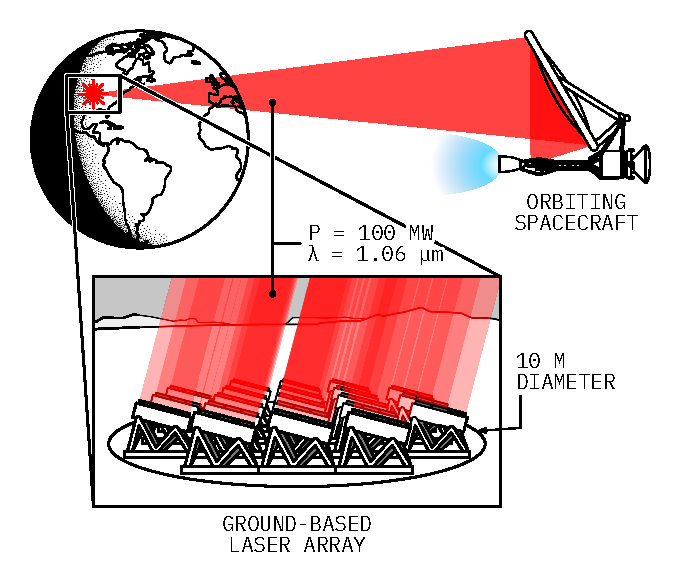
\includegraphics[width=0.4\textwidth]{assets/2 background/ltp_architecture.pdf}
            \caption{LTP architecture (\textcite{duplayArgonLaserPlasmaThruster2024a})}
            \label{fig:LTP architecture}
        \end{figure}

        Initially, hydrogen propellant is introduced in the thrust chamber of the vehicle. The laser is focused inside the chamber (see \autoref{fig:LTP system overview}) and is absorbed by the gas via inverse Bremsstrahlung, creating a Laser-Supported Plasma (LSP) core. Colder hydrogen flows around the LSP core and is heated by it to \qty{10000}{K}. The hot gas is then exhausted through a conventional converging-diverging nozzle at the exhaust velocity, imparting thrust to the vehicle.

        \begin{figure}[!ht]
            \centering
            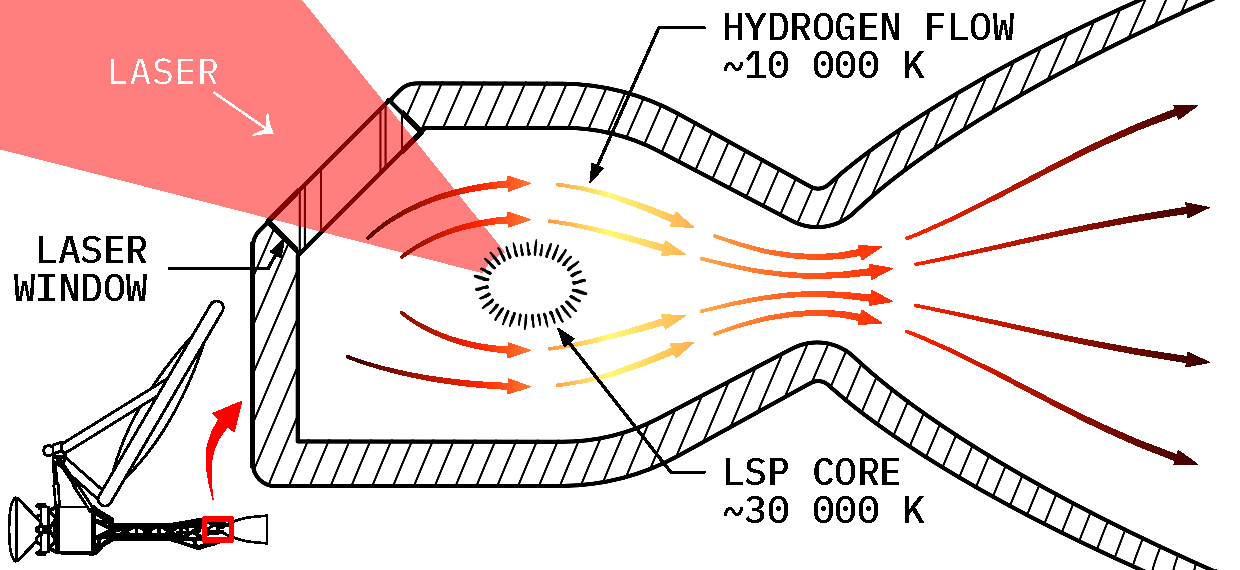
\includegraphics[width=0.6\textwidth]{assets/2 background/chamber.pdf}
            \caption{Overview of LTP system (\textcite{duplayArgonLaserPlasmaThruster2024a})}
            \label{fig:LTP system overview}
        \end{figure}

        In a conventional chemical rocket engine, the energy source is the oxidizer and the fuel, which are reacted together to release energy. They are transported with the rocket and set the temperature of the combustion reaction (typically \qtyrange{2000}{3000}{K}), which is directly related to the exhaust velocity.
        
        Separating the power source used for propulsion (here, the laser) from the spacecraft itself allows crucial weight savings, either increasing the payload mass fraction or decreasing transit time. Using a laser also allows for much greater thrust chamber temperatures than chemical propulsion, as the temperature of these plasmas is typically \qtyrange{15000}{30000}{K}. This gives in turn greater exhaust velocities. This propulsion method could therefore be an order of magnitude more efficient than our current rocket engines if certain engineering problems can be solved.

        Increasing the amount of energy deposited by the laser into the propellant remains a topic of active research and is a significant hurdle for the operational use of LTP. The two main conversion efficiencies are:
        \begin{enumerate}
            \item Absorption of the laser energy by the plasma
            \item Heat transfer from the plasma to the propellant
        \end{enumerate}
        A selection of past LSP experiments will now be presented, with an emphasis on these efficiencies. As the efficiencies chosen are different from source to source, they will be defined where applicable.
    
    \section{Literature review}

        %Russian work: 1960s-2000s?

        The experimental basis of LTP was developed by \textcite{generalovContinuousOpticalDischarge1970} in 1970. For the first time, an LSP was generated with a \qty{150}{W} \ce{CO2} laser operating at a \qty{10.6}{μm} wavelength. In this case, the LSP was initiated by a second, \qty{10}{kW} pulsed \ce{CO2} laser.
        
        %American work: 1970s-1990s?

        Work was done in the mid-1970s by \textcite{shojiLaserheatedRocketThruster1977,shojiPerformanceHeatTransfer1976a} to design a small-scale \qty{10}{kW} and full-scale \qty{5000}{kW} LTP engine. Carbon-seeded hydrogen was proposed to capture the plasma's radiation, which was mostly in the UV wavelength. \qty{20}{\%} of the laser power would be lost by convection and radiation to the walls in the \qty{10}{kW} thruster, with an additional \qty{5}{\%} of laser power lost by radiation through the thruster window. However, these engines were not tested. The \qty{10}{kW} prototype (\autoref{fig:Shoji apparatus}) was built and delivered to NASA at the conclusion of their effort.
        \begin{figure}[!ht]
            \centering
            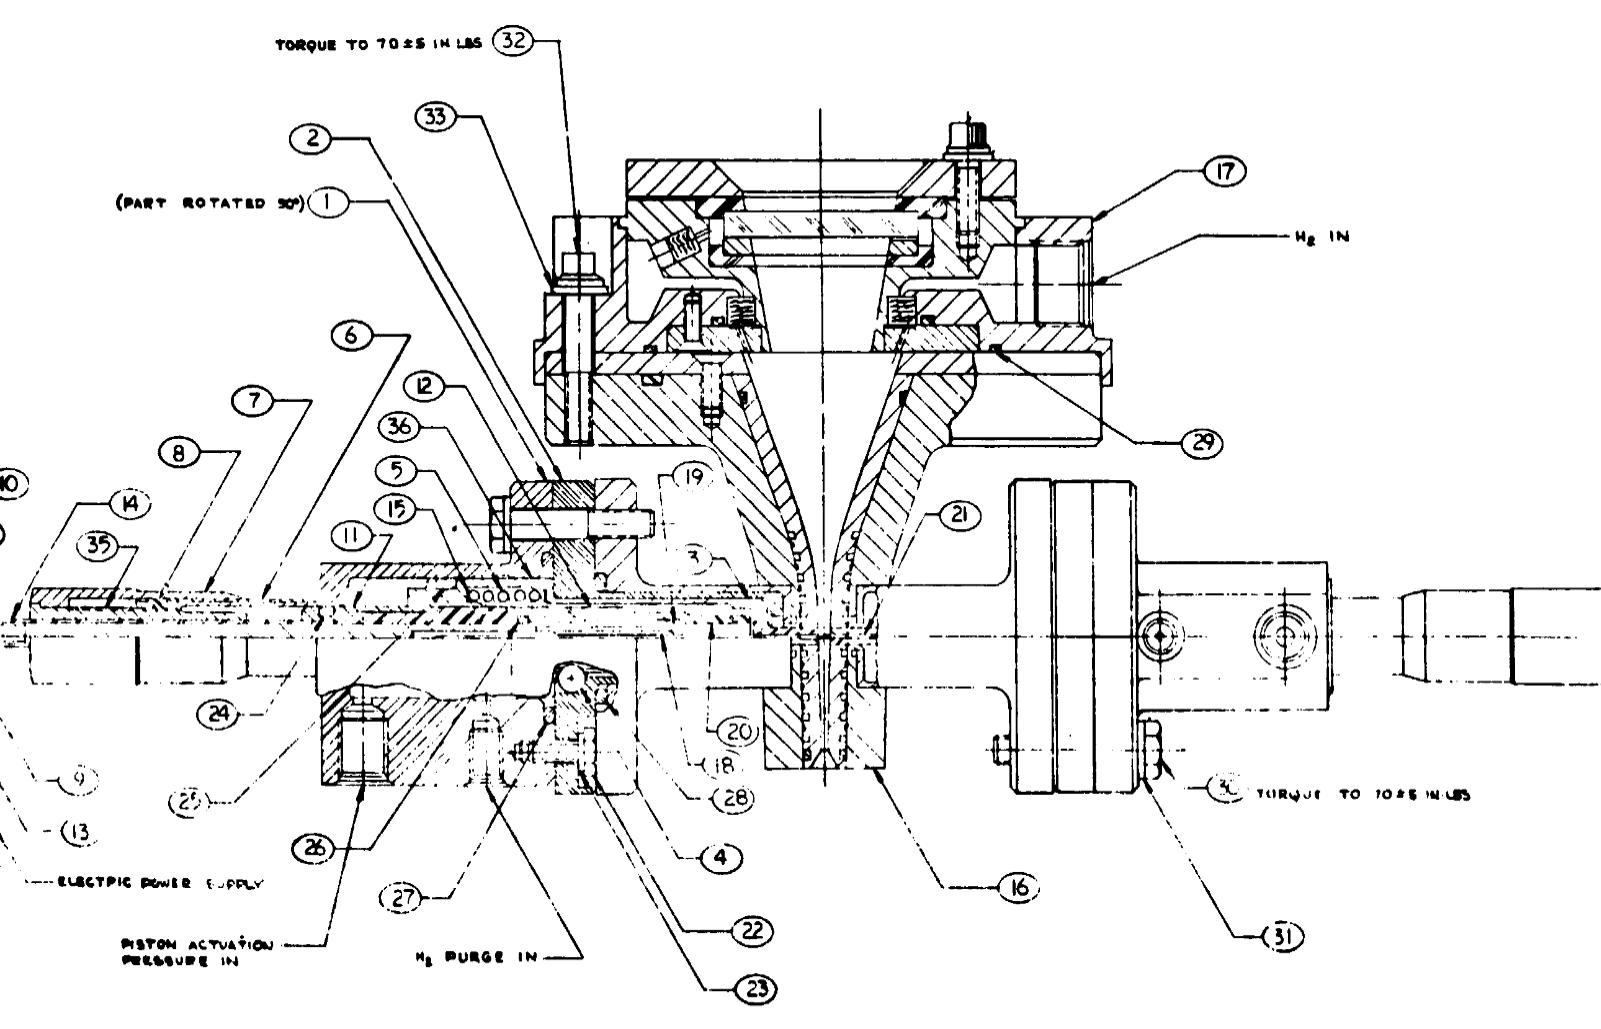
\includegraphics[width=0.5\textwidth]{assets/2 background/Shoji cross-section.png}
            \caption{Cross-section drawing of \qty{10}{kW} thruster from \textcite{shojiLaserheatedRocketThruster1977} (original is of poor quality)}
            \label{fig:Shoji apparatus}
        \end{figure}

        In the 1980s, \textcite{keeferPowerAbsorptionLasersustained1986a} studied LSP in a forced convective flow environment. Using a \qty{1.5}{kW} \ce{CO2} laser with power levels of \qtyrange{360}{840}{W} and pressures of \qtyrange{1.3}{2.3}{atm}, with varying argon flow velocities, the temperature field of the plasma was measured. From the temperature field, and assuming local thermodynamic equilibrium, the power absorbed by the plasma and the power radiated from it can be calculated.
        \begin{figure}[!ht]
            \centering
            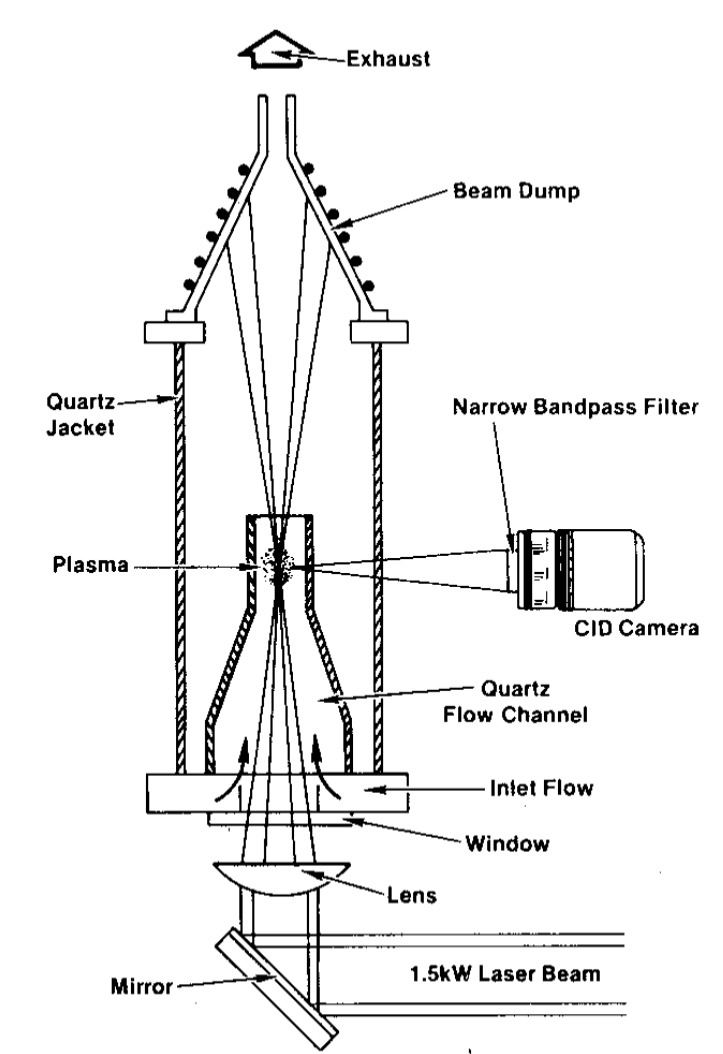
\includegraphics[width=0.4\textwidth]{assets/2 background/UTSI (Keefer) Apparatus.png}
            \caption{Experimental apparatus from \textcite{keeferPowerAbsorptionLasersustained1986a}}
            \label{fig:Keefer apparatus}
        \end{figure}
        \autoref{fig:Keefer apparatus} shows the apparatus used for these measurements. An inner quartz flow channel contained the plasma, while an outer quartz jacket contained the pressure. The plasma was initiated by laser heating of a tungsten rod, which was removed after initiation. Downstream, a water-cooled copper beam dump absorbed the energy of the laser and the heated argon flow, but it was not used for any measurements. The plasma's temperature was obtained through analyzing digital images. This temperature field was then used to calculate the power absorption and the radiation loss. The power absorbed by the plasma was between \qtyrange{23}{61}{\%} of incident laser power, while the radiation loss was between \qtyrange{51}{80}{\%} of the absorbed power.

        Contemporary to \textcite{keeferPowerAbsorptionLasersustained1986a}, Mazumder and Krier headed a group at the University of Illinois that advanced the field of LTP. \textcite{krierContinuousWaveLaser1986a} reported laser absorption in an argon plasma approaching \qty{80}{\%}. \autoref{fig:Krier apparatus} shows the apparatus that was used by \textcite{krierContinuousWaveLaser1986a}, \textcite{zerkleLasersustainedArgonPlasmas1990}, and \textcite{chenEmissionSpectroscopyCw1989a}. This vertical cylindrical flow chamber was made of 304 steel and had an internal diameter of 5 inches. A water-cooled calorimeter was used as a beam dump for the \qty{10}{kW} \ce{CO_2} laser. The laser energy not collected by the calorimeter (beam dump) was assumed to be absorbed by the plasma, as the radiation reflected off the plasma is less than \qty{2}{\%} at these electron number densities. Moveable thermocouples gave a two-dimensional map of the flow surrounding the plasma core. The direct laser heating of the thermocouples and their carriage was taken into account.
        \begin{figure}[!ht]
            \centering
            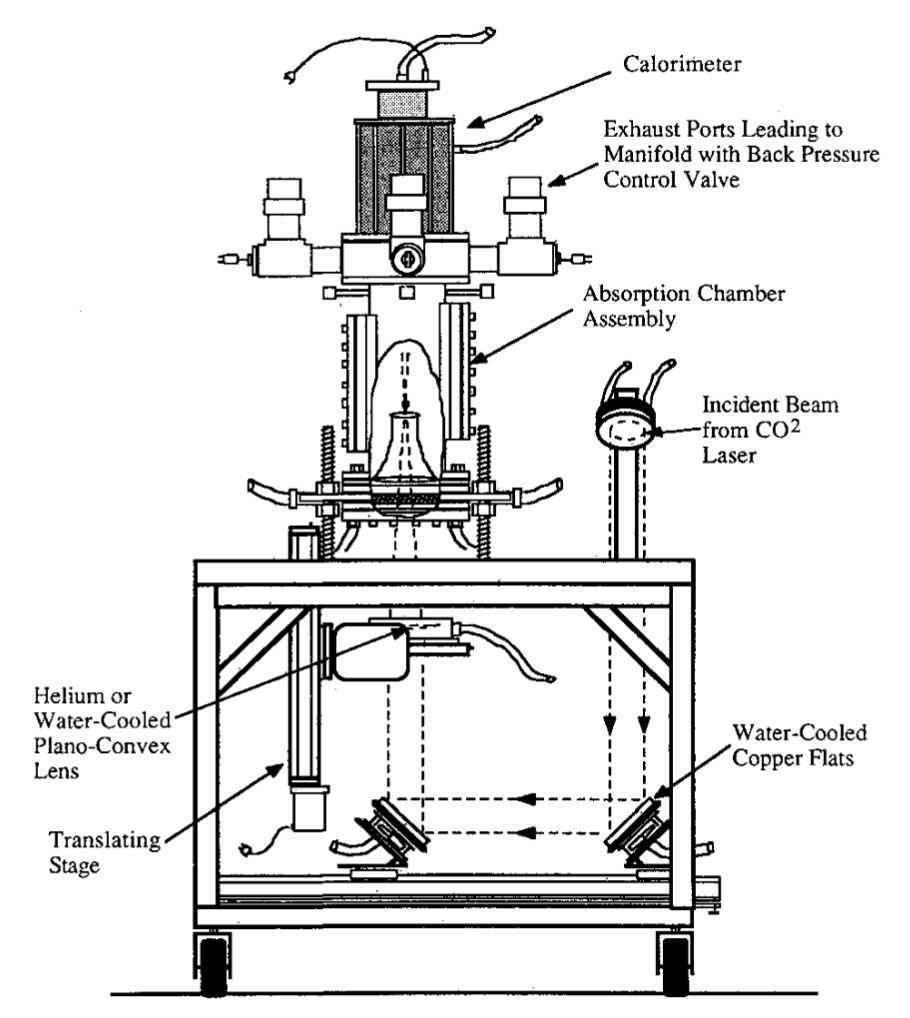
\includegraphics[width=0.5\textwidth]{assets/2 background/Illinois (Krier) Apparatus.png}
            \caption{Experimental apparatus from \textcite{zerkleLasersustainedArgonPlasmas1990}}
            \label{fig:Krier apparatus}
        \end{figure}
        With the two-dimensional temperature map, the change in enthalpy at the exit plane was calculated, giving the amount of laser energy retained by the gas. Thermal efficiency was between \qtyrange{6}{25}{\%}, with radiative losses of \qty{64}{\%} and \qty{30}{\%}, respectively. Thermal efficiency was defined as:
        \[\eta_\mathrm{th} =  \frac{\text{Power retained by the gas}}{\text{Incident laser power}}\]
        The minimum maintenance intensity of the plasma was also estimated at \qtyrange{0.1}{0.3}{MW/cm^2}.

        Further work by \textcite{zerkleLasersustainedArgonPlasmas1990} with the apparatus shown in \autoref{fig:Krier apparatus} reported absorption from \qtyrange{55}{97}{\%} and thermal efficiency from \qtyrange{11}{46}{\%}. This was done in \qtylist{1 2.5}{atm} of flowing argon, with laser powers up to \qty{7}{kW}. \textcite{chenEmissionSpectroscopyCw1989a} again increased the thermal efficiency of this apparatus, with \qtyrange{41}{62}{\%} of the laser energy being retained by the gas as thermal energy. This was among the highest thermal efficiencies measured by an LSP experiment. Here, \qty{86}{\%} of the laser's energy is absorbed by the LSP. This was attained with a \qty{5}{kW} \ce{CO2} laser, with flow speeds between \qtyrange{2}{10}{m/s}. They discuss that greater thermal efficiency is due to greater laser power, a high enough flow speed, and a greater laser focusing $f$ number.

        Based on work by the Illinois group, an LTP engine demonstrator was tested in 1995 by \textcite{blackLaserPropulsion10kW1995} with a \qty{10}{kW} \ce{CO2} laser. This was planned to be a step towards a full-scale thruster. More than 100 thruster firings were completed, lasting 1 to 2 minutes each. The \qty{10}{kW} thruster is presented in \autoref{fig:Black apparatus}. It is mounted in a vacuum chamber to a thrust measurement assembly. Efficiency was calculated from:
        \[ \eta = \frac{F^2}{2 \dot{m} P_\mathrm{L}} \]
        with $P_\mathrm{L}$ the input laser power at the thruster window. Both argon and hydrogen were used. Argon propellant produced \qty{200}{s} of $I_\mathrm{sp}$ and a peak efficiency of 0.24. With hydrogen propellant, an $I_\mathrm{sp}$ of \qty{350}{s} and a peak efficiency of 0.37 were reported.
        \begin{figure}[!ht]
            \centering
            \begin{subfigure}[t]{0.3\textwidth}
                \centering
                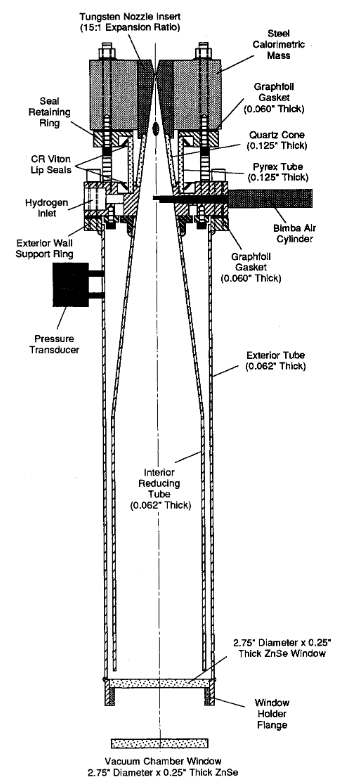
\includegraphics[width=\textwidth]{assets/2 background/BlackKrier thruster.png}
                \caption{\qty{10}{kW} thruster}
                \label{fig:Black apparatus}
            \end{subfigure}
            \hfill
            \begin{subfigure}[t]{0.45\textwidth}
                \centering
                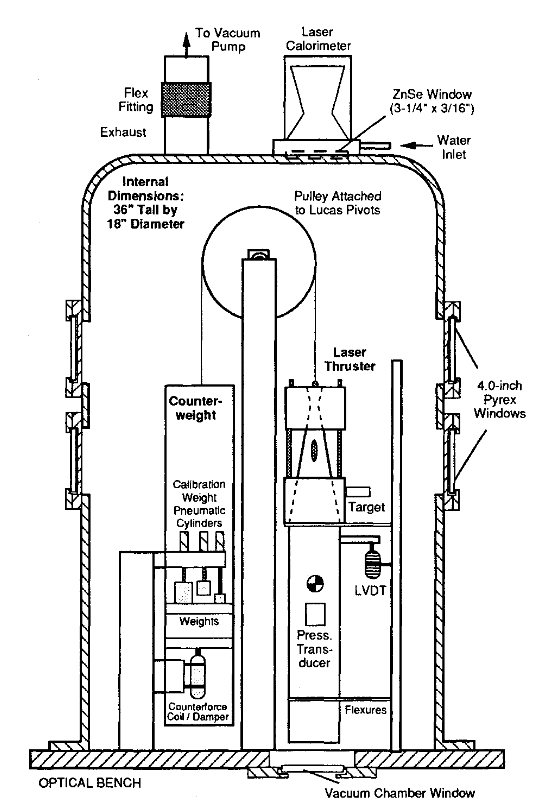
\includegraphics[width=\textwidth]{assets/2 background/Black thrust measurement assy.png}
                \caption{Thrust measurement assembly}
                \label{fig:Black thrust measurement}
            \end{subfigure}
            \caption{Apparatus used in \textcite{blackLaserPropulsion10kW1995}}
            \label{fig:Black apparatussies}
        \end{figure}
        A preliminary design for the full-scale \qty{100}{kW} thruster was also presented, with a predicted specific impulse of \qty{1000}{s}, thrust of \qty{4.5}{N} and a conversion efficiency of \qty{80}{\%}.

        %Chinese and Japanese work: 1980s-2020s

        In the early 2000s, \textcite{toyodaThrustPerformanceCW2002} built and tested two different thruster models, presented in \autoref{fig:Toyoda apparatussies}. These thrusters, using argon or nitrogen heated by LSP, were powered by a \qty{2}{kW} \ce{CO2} laser. The LSPs were initiated by a retractable tungsten rod at the laser's focus. Thrust measurements were done both in atmospheric pressure and in vacuum. This comparative study showed that confining the plasma into a smaller chamber increased thrust and therefore, efficiency. \textcite{toyodaThrustPerformanceCW2002} defined the energy conversion efficiency as the amount of laser power that is converted into usable kinetic energy for thrust. It is calculated as\footnote{As mentioned by \textcite{duplayArgonLaserPlasmaThruster2024a}, there appears to be a typographical error in the reference as the units are inconsistent. The corrected equation is presented here.}:
        \[ \eta_\mathrm{e} =  \frac{F^2_\mathrm{hot} -F^2_\mathrm{cold}}{2 \dot{m} P}\]
        Where $F_\mathrm{hot}$ is the thrust with laser on, $F_\mathrm{cold}$ is the cold flow thrust (laser off) and $P$ is incident laser power. An energy conversion efficiency of 37\% and an $I_\mathrm{sp}$ of \qty{113}{s} were measured with the second model \autoref{fig:Toyoda apparatus 2} in vacuum with argon propellant. The pressure ratio, defined as the chamber pressure divided by the nozzle exit pressure, was 420. A water cooling system measured the heat loss to the walls to be 55\% of incident laser power, with a final 8\% being ``other loss". Heat loss to the walls was expected to be recycled with regenerative cooling in a real-world application.

        \begin{figure}[!ht]
            \centering
            \begin{subfigure}[t]{0.45\textwidth}
                \centering
                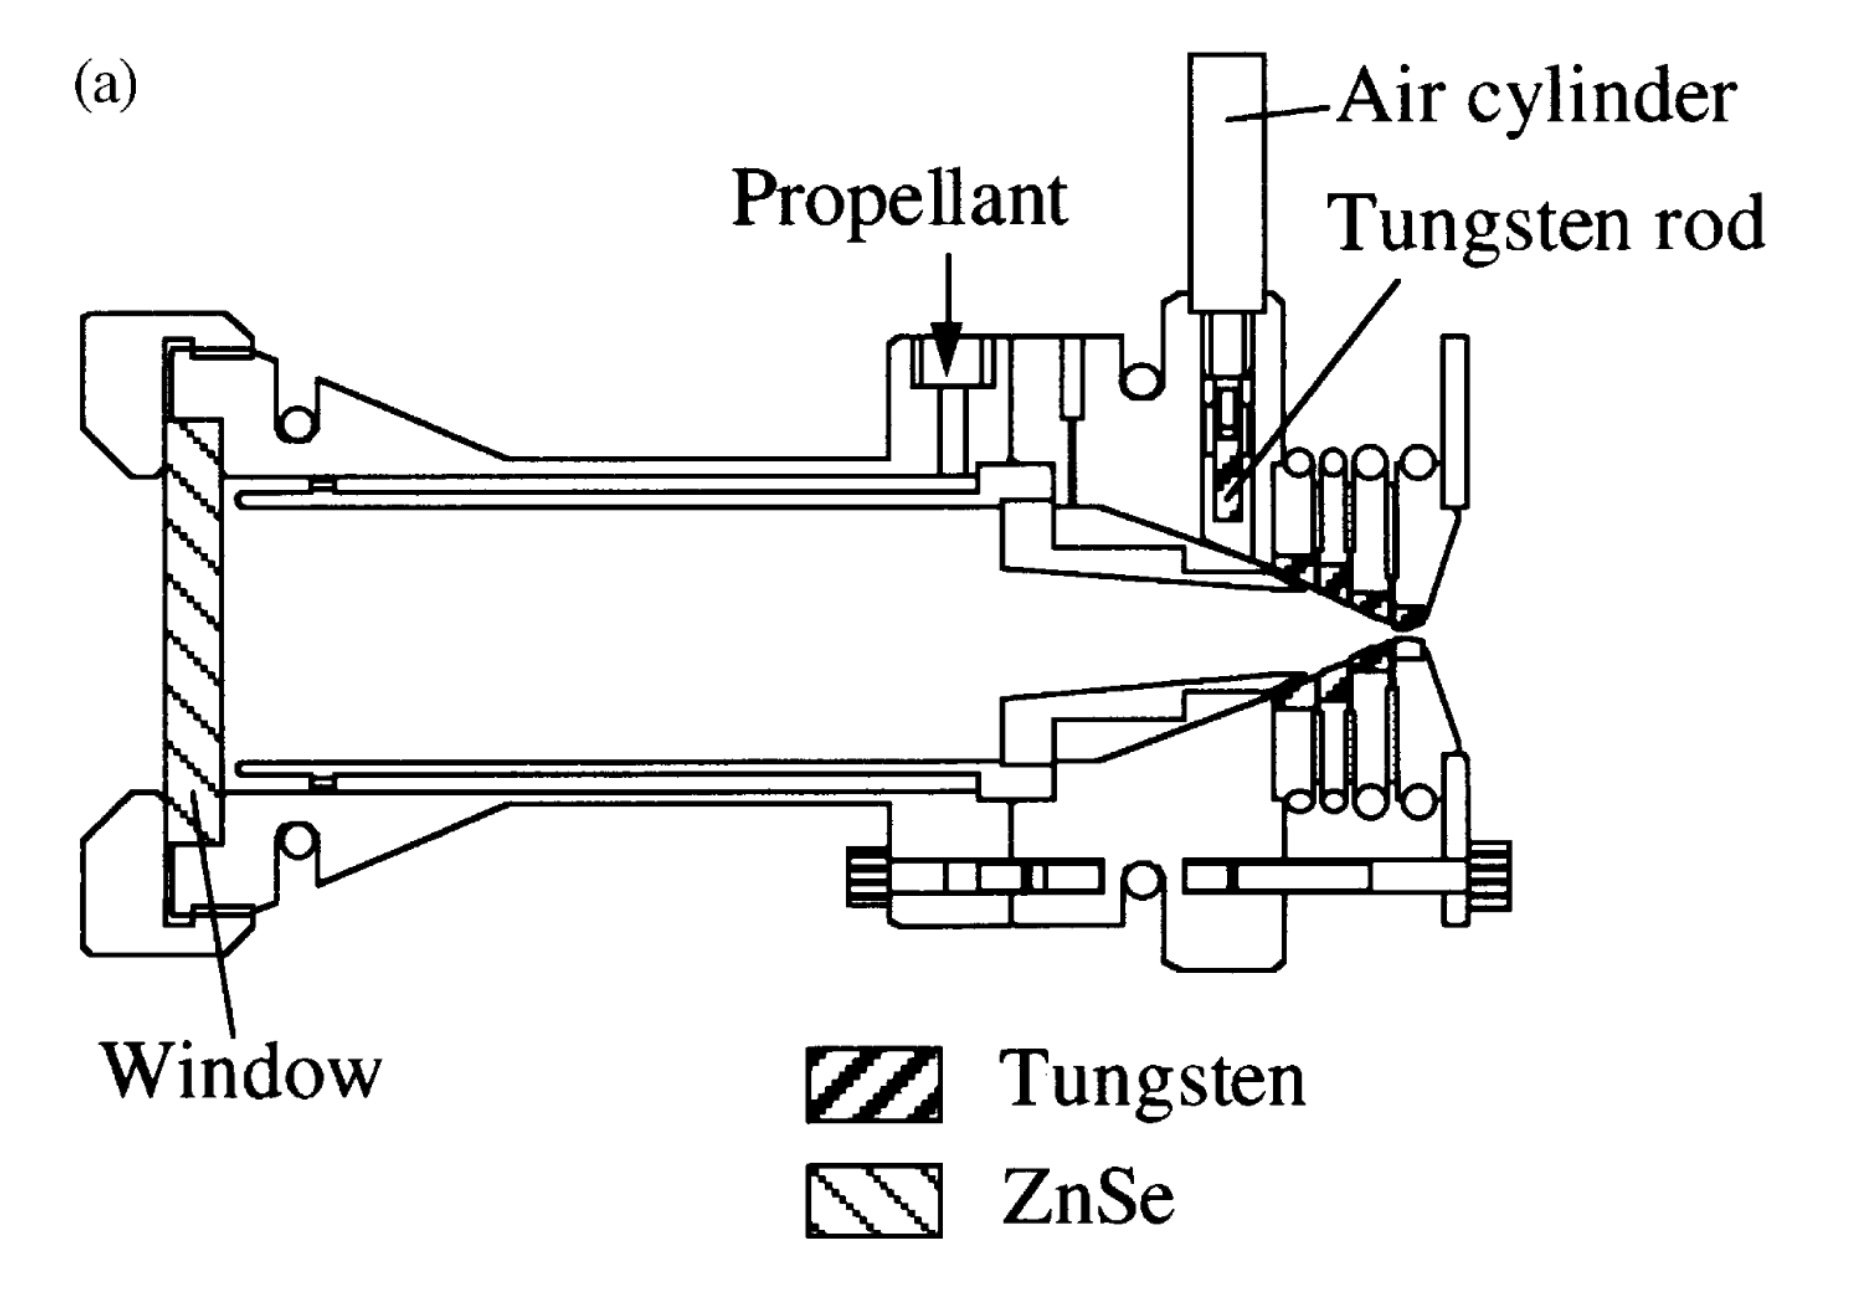
\includegraphics[width=\textwidth]{assets/2 background/Toyoda apparatus model 1.jpg}
                \caption{Model I}
                \label{fig:Toyoda apparatus 1}
            \end{subfigure}
            \hfill
            \begin{subfigure}[t]{0.45\textwidth}
                \centering
                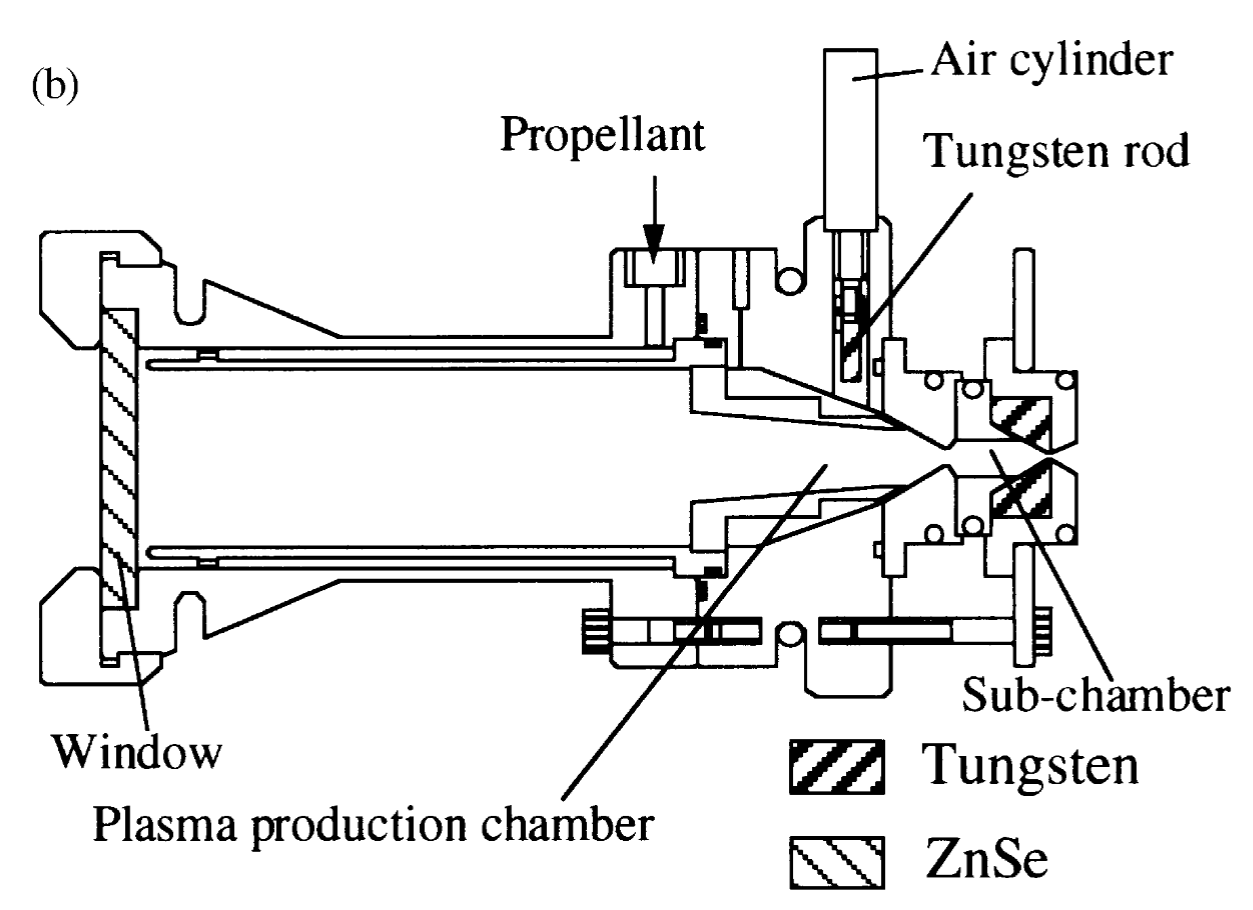
\includegraphics[width=\textwidth]{assets/2 background/Toyoda Apparatus model 2.png}
                \caption{Model II}
                \label{fig:Toyoda apparatus 2}
            \end{subfigure}
            \caption{Two thruster models from \textcite{toyodaThrustPerformanceCW2002}}
            \label{fig:Toyoda apparatussies}
        \end{figure}

        \textcite{luCharacteristicDiagnosticsLaserStabilized2022a} investigated LSP for lighting applications instead of propulsion. Therefore, an emphasis was made on spectroscopy measurements. A \qty{300}{W} fiber laser at a wavelength of \qty{1080}{nm} was focused to a \qty{50}{μm} diameter spot in a high pressure chamber.
        \begin{figure}[!ht]
            \centering
            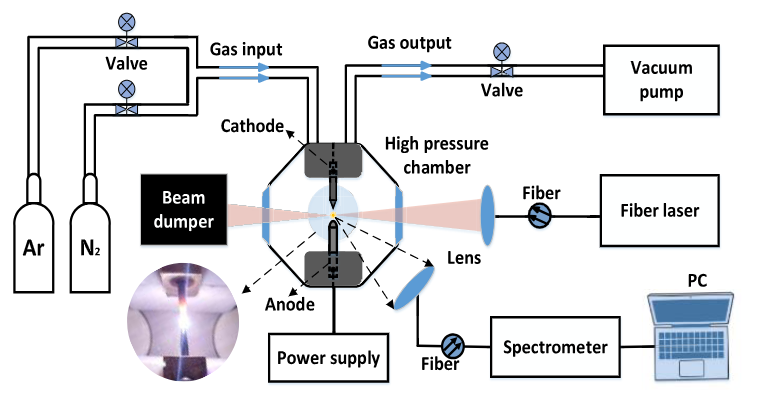
\includegraphics[width=0.7\textwidth]{assets/2 background/Lu apparatus.png}
            \caption{Experimental setup from \textcite{luCharacteristicDiagnosticsLaserStabilized2022a}}
            \label{fig:Lu apparatus}
        \end{figure}
        Argon was used, with pressures between \qtyrange{10}{20}{bar}. A lower initiation power (\qty{117}{W}) than other studies was achieved at \qty{20}{bar}. This was attributed to the smaller focus delivering a greater photon flux. \ce{N2} was later added between \qtyrange{0.1}{1.0}{\%}. As expected, increasing the laser power or the gas pressure was found to increase the radiation intensity of the LSP. However, adding \ce{N2} reduced both the electron temperature and electron density of the LSP, reducing its radiation intensity.

        Seeding the propellant with another species has been discussed as a way to increase the energy absorption into the working fluid of an LTP engine. LSPs in pure methane and methane-seeded gasses have been investigated by \textcite{kameiMethaneMethaneXenon2020}. Methane dissociates into hydrogen and carbon with the high temperature of the LSP. As mentioned with \textcite{shojiLaserheatedRocketThruster1977}, carbon particles would absorb the LSP's UV radiation.  A \qty{1.1}{kW} diode laser at a wavelength of \qty{940}{nm} was beamed into a high-pressure chamber fitted with arc initiation electrodes. The gap between these electrodes was \qty{1}{mm}. A CCD type spectrometer recorded emission spectra of the initiation arc discharge and of the LSP. LSPs in three different gasses were attempted: pure methane, methane-argon, and methane-xenon.
        
        In methane at \qty{0.1}{MPa}, soot formation between the electrodes prevented LSP initiation. The spectrometer confirmed the dissociation of methane, as line spectra of carbon and hydrogen were observed at the initiation arc. Initiation was also unsuccessful in argon-methane with a pressure between \qtyrange{0.1}{0.3}{MPa} and a methane volume fraction between \qtyrange{20}{60}{\%}. LSP was successfully generated in methane-xenon, with a lower threshold power (\qty{850}{W}) than in pure xenon. The partial pressure of methane was between \qtyrange{0.02}{0.6}{MPa}, with a partial pressure of xenon of \qty{0.10}{MPa}.

        \textcite{takanoDemonstrationDiodeLasersustained} used a diode laser emitting simultaneously at \qty{927}{nm} and \qty{951}{nm} to generate LSPs in argon. This resulted in an $I_\mathrm{sp}$ of \qty{105}{s} and a thrust efficiency of \qty{8}{\%}. This $I_\mathrm{sp}$ was calculated from the plenum pressure when the laser was on. They define thrust efficiency as:
        \[
        \eta = \frac{g_0 I_\mathrm{sp} (F_\mathrm{hot}-F_\mathrm{cold})}{2 P_\mathrm{laser}}
        \]
        Two setups were used: the LSP generation chamber previously used by \textcite{kameiMethaneMethaneXenon2020} (\autoref{fig:Takano LSP generation chamber}) and an LSP thruster (\autoref{fig:Takano LSP thruster}).
        \begin{figure}[!ht]
            \centering
            \begin{subfigure}[t]{0.45\textwidth}
                \centering
                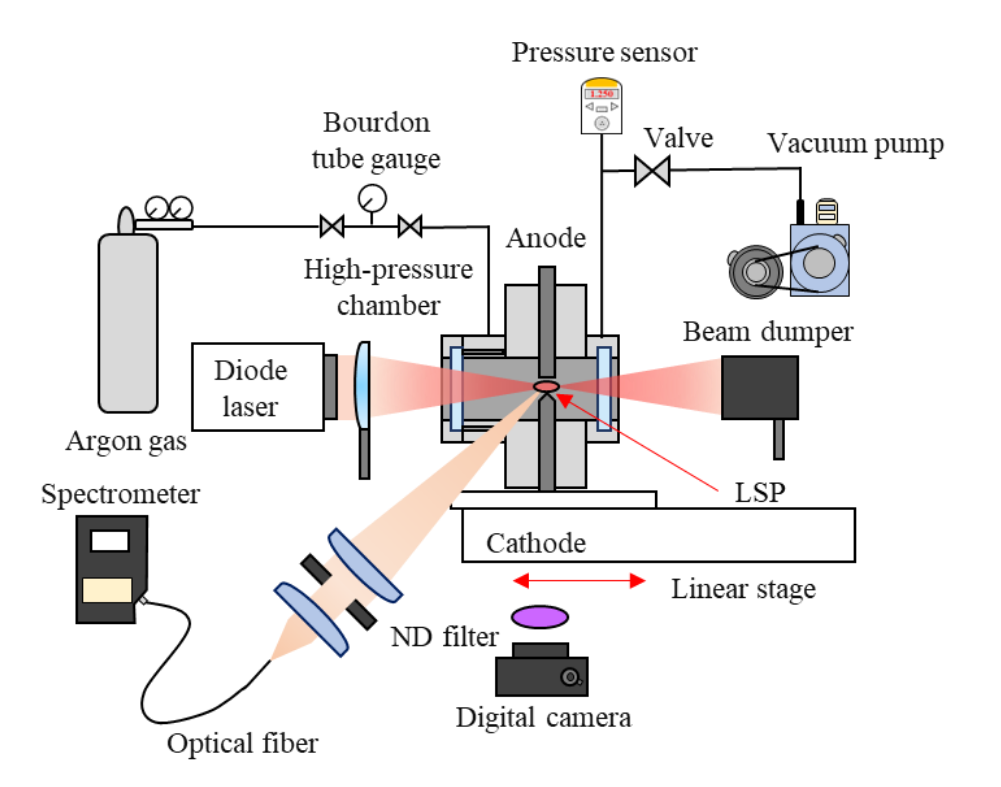
\includegraphics[width=\textwidth]{assets/2 background/Takano LSP chamber.png}
                \caption{LSP generation chamber and systems}
                \label{fig:Takano LSP generation chamber}
            \end{subfigure}
            \hfill
            \begin{subfigure}[t]{0.45\textwidth}
                \centering
                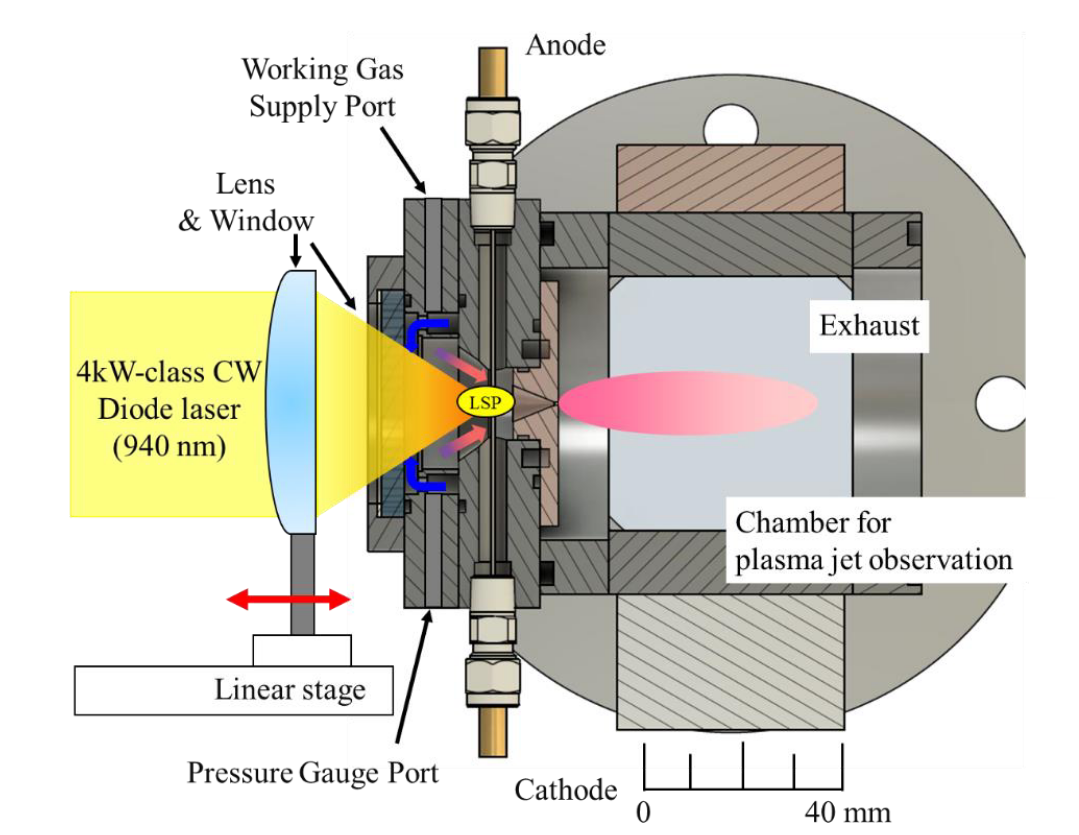
\includegraphics[width=\textwidth]{assets/2 background/Takano LSP thruster.png}
                \caption{LSP thruster}
                \label{fig:Takano LSP thruster}
            \end{subfigure}
            \caption{LSP setups from \textcite{takanoDemonstrationDiodeLasersustained}}
            \label{fig:Takano apparatussies}
        \end{figure}
        The LSP chamber was used to determine the effect of various F-numbers on the argon LSP. The thruster has an interchangeable copper throat, with diameters of \qty{0.7}{mm} and \qty{1.0}{mm}. In both setups, electric arc initiation was used. Once initiated in the thruster, the LSP is moved toward the nozzle with the lens mounted on a motorized stage. It was found that moving the LSP this way increased the heat exchange with the propellant. Thrust was calculated by using the pressure measurements inside the thruster's heating chamber.

        %Canadian work: 2020s  

        \textcite{duplayArgonLaserPlasmaThruster2024a} used a \qty{3}{kW} pulsed fiber laser to create LSPs in static and flowing argon. In static argon, about \qty{80}{\%} of the laser energy was being absorbed by the plasma, with approximately \qty{15}{\%} of the laser energy heating the bulk gas. This was done between \qtyrange{5}{20}{bar}.

    \section{Summary and direction of work in this thesis}
        
        From the literature review, \autoref{tab:lit review summary} and \autoref{tab:efficiencies} were compiled. Most studies have used \ce{CO2} lasers with a wavelength of \qty{10.6}{μm}. As a laser beam advances in space, it diffracts. This leads to a larger spot size the farther it is focused, even with ideal optics. The range $L$ at which the laser's spot size is equal to its emitter size is derived by \textcite{lubinRoadmapInterstellarFlight2016}:
        \[
            L = \frac{dD}{2\lambda\alpha}
        \]
        With $d$ the diameter of the laser aperture, $D$ the diameter of the laser receiver, and $\alpha = 1.22$ for a circular array, deriving from the first zero of the $J_1$ Bessel function. A smaller wavelength ($\lambda$) gives a larger value of $L$, as the beam diverges less. Use of a \ce{CO2} laser for power beaming to a remote target for propulsion applications is limited to ground-to-orbit launch. However, high power fiber lasers emitting near \qty{1}{μm} have recently become readily available. Being able to beam energy ten times farther than \ce{CO2} lasers, fiber lasers make laser propulsion more feasible.

        \begin{table}[!ht]
            \centering
            \caption{Summary of a selection of past LSP experiments. $\lambda$: wavelength, $P$: maximum laser power, $p$: pressure, $I_\mathrm{sp}$: maximum specific impulse, $F_\mathrm{T}$: maximum thrust}
            \label{tab:lit review summary}
            \begin{tabularx}{\textwidth}{@{}>{\small}X<{\raggedright}lXXrXXrr<{\raggedright}@{}}
            \toprule
            {\normalsize LSP   Facility} & Year & Laser & $\lambda$ [\unit{\um}] & $P$ [kW] & Gas & $p$ [bar] & $I_\mathrm{sp}$ [s] & $F_\mathrm{T}$ [N]  \\ \midrule
            \textcite{generalovContinuousOpticalDischarge1970}        &1970&\ce{CO_2}&10.60&0.15 &\ce{Xe}           & 1.0–10.1  & -     &  -   \\
            \textcite{keeferPowerAbsorptionLasersustained1986a}       &1986&\ce{CO_2}&10.60&0.84 &\ce{Ar}           & 1.3–2.3   & -     &  -   \\
            \textcite{krierContinuousWaveLaser1986a}                  &1986&\ce{CO_2}&10.60&10.0  &\ce{Ar}            &   1.1–3.5 & -     & -\\
            \textcite{zerkleLasersustainedArgonPlasmas1990}           &1988&\ce{CO_2}&10.60&7.0   &\ce{Ar}            &  1.0–2.5  & -     &- \\
            \textcite{chenEmissionSpectroscopyCw1989a}                &1989&\ce{CO_2}&10.60&5.0   &\ce{Ar}            &    1.0    & -     & -    \\
            \textcite{blackLaserPropulsion10kW1995}                   &1995&\ce{CO_2}&10.60&10.0  &\ce{Ar}            & 0.9–2.6   & 200   & 7.0 \\
                                                                      &    &\ce{CO_2}&10.60&10.0  &\ce{H_2}           & 1.9–3.4    &  350  & 3.6 \\
            \textcite{toyodaThrustPerformanceCW2002}                  &2002&\ce{CO_2}&10.60&2.0   &\ce{Ar}, \ce{N_2}  & 2.0–5.6   & 113   & 0.44 \\
            \textcite{luCharacteristicDiagnosticsLaserStabilized2022a}&2022&Fiber    &1.08 &0.30 &\ce{Ar}, \ce{N_2} & 10.0–20.0  & -     & -    \\ 
            \textcite{takanoDemonstrationDiodeLasersustained}         &2024&Diode    &0.927 and 0.951 &4.4 &\ce{Ar} & 6.0–20.0     & 105   & -    \\
            \textcite{duplayArgonLaserPlasmaThruster2024a}            &2024&Fiber    &1.07  & 3.0 &\ce{Ar}            &   3.0–20.0    & -     & - \\
            \bottomrule
            \end{tabularx}
        \end{table}

        \begin{table}[!ht]
            \centering
            \caption{Comparative table of experimental LTP thruster efficiencies}
            \label{tab:efficiencies}
            \begin{tabularx}{\textwidth}{@{}>{\small}X<{\raggedright} X l r@{}}
            \toprule
            {\normalsize LSP   Facility}   & Fraction of laser power absorbed  & Efficiency formula & Value of efficiency \\ \midrule
            \textcite{keeferPowerAbsorptionLasersustained1986a}   & 0.23–0.61      &          -        &                 -          \\
            \textcite{krierContinuousWaveLaser1986a}       & 0.50–0.80         & $\eta_\mathrm{th} =  \frac{\text{Power retained by the gas}}{\text{Incident laser power}}$ &  0.06–0.25 \\
            \textcite{zerkleLasersustainedArgonPlasmas1990}       & 0.55–0.97   &         $\eta_\mathrm{th} =  \frac{\text{Power retained by the gas}}{\text{Incident laser power}}$ &  0.11–0.46 \\
            \textcite{chenEmissionSpectroscopyCw1989a}          & 0.86                      &  $\eta_\mathrm{th} =  \frac{\text{Power retained by the gas}}{\text{Incident laser power}}$  &  0.41-0.62  \\
            \textcite{blackLaserPropulsion10kW1995}       &  -  & $ \eta = \frac{F_\mathrm{hot}^2}{2 \dot{m} P_\mathrm{L}} $& 0.18–0.24 (\ce{Ar}), 0.25–0.37 (\ce{H_2})     \\
            \textcite{toyodaThrustPerformanceCW2002}    & -                      & $ \eta_\mathrm{e} =  \frac{F^2_\mathrm{hot} -F^2_\mathrm{cold}}{2 \dot{m} P} $     &   0.37 \\
            \textcite{takanoDemonstrationDiodeLasersustained}  &       -       & $ \eta = \frac{g_0 I_\mathrm{sp} (F_\mathrm{hot}-F_\mathrm{cold})}{2 P_\mathrm{laser}} $ & 0.08 \\ 
            \textcite{duplayArgonLaserPlasmaThruster2024a}  &  0.79&  $\eta_\mathrm{th} =  \frac{\text{Power retained by the gas}}{\text{Incident laser power}}$ & 0.15 \\
            \bottomrule
            \end{tabularx}
        \end{table}
        
        To increase thermal efficiency, \textcite{chenEmissionSpectroscopyCw1989a} suggest:
        \begin{enumerate}
            \item A greater laser power, which gives greater inverse bremsstrahlung absorption coefficient and longer absorption path length;
            \item A high enough flow speed to push the LSP back to the laser focus, but not too fast as to blow the plasma out;
            \item A greater laser focusing $f$ number, creating a longer and narrower plasma. This increases the probability that a photon from the laser will be absorbed by the plasma and reduces the radiation loss.
        \end{enumerate}

        For a small-scale, demonstration thruster, $I_\mathrm{sp}$ values near \qty{100}{s} can be expected, with thrust values under \qty{1}{N}, as was found by \textcite{toyodaThrustPerformanceCW2002} and \textcite{takanoDemonstrationDiodeLasersustained}.
        
        The objective of this research project will be to test a Version 1 (V1) lab-scale LTP thruster, as well as design and test an improved Version 2 (V2) thruster. These will be both powered by a \qty{1.07}{μm} fiber laser. This project will mainly build upon the experimental research started by \textcite{duplayArgonLaserPlasmaThruster2024a} with the V1 thruster.

        % Goal: advance experimental understanding of LTP engine concept, validate spark initiation, validate and characterise the V2 thruster under qcw pulsed operation, and confirm CW operation of the V2 thruster
        % Goal: demonstrate survivability of V2 under high (3kW) laser power
        % Goal: a practical guide for future laser rocketeers to develop their LTP engines, including how to achieve reliable spark initiation
        
        % % Link to next chapter, modelling c_p
        % To attempt to explain experimental results, a 0D heat transfer model will be presented in the next chapter.
        % certain thermodynamic properties of the gasses used will be characterized. Notably, the modelling of heat capacity
